\subsection*{Fundamental: Feedback loops and Ripples\label{sec:feedback-loop-and-ripples}}

%When there is a lack of input from customers or users, then someone has to decide.


A feedback loop exists when a decision-maker experiences the harms and benefits of their decision. Decisions that lack a feedback loop still have consequences for the decision-maker, in that potential future decisions are altered or limited.\footnote{In Street-Level Bureaucracy~\cite{1983_Lipsky} Lipsky discusses feedback loops in chapter~4 on page~40.}


Virtuous cycles and vicious cycles are rare in bureaucratic organizations because there are rarely mechanisms for feedback loops. 
Instead, there are \iftoggle{glossarysubstitutionworks}{\glspl{ripple}}{ripples} -- propagation of consequences for other people's schedules, 
altering what is possible for other people, and creating dependent tasks to be carried out by people other than the decision-maker.


The weak feedback mechanisms for a bureaucrat are reputation (subject to spin)
\index{reputation}
and rarely enforced retroactive accountability in the form of the question, ``What did you know and when did you know it?''
%Reputation is social.
Retroactive accountability depends on written records from meeting notes, emails, agendas, and reports. Reducing the potential for retroactive accountability is one motive for bureaucrats avoiding written records for decisions and policies.

When there are multiple competing objectives among stakeholders in a 
\href{https://en.wikipedia.org/wiki/Zero-sum_game}{zero-sum}
\index{Wikipedia!zero-sum game@\href{https://en.wikipedia.org/wiki/Zero-sum_game}{zero-sum game}}\iftoggle{WPinmargin}{\marginpar{$>$Wikipedia: zero-sum game}}{}
use of resources (my win is your loss), how can you determine what's best? In some domains there are feedback loops to guide progress. When feedback loops are weak or not present,  the most powerful stakeholder (potentially distinct from the biggest or loudest) will dominate. 

\subsubsection*{Approvals and Justifications}

Because of the lack of quantitative feedback loops for bureaucrats, there is significant interest in documenting justification, proactive monitoring, reporting, and retroactive assessment. Each of those activities creates more administrivia. Deepening your Process Empathy involves looking for feedback loops (which are rare) and understanding what arises in place of feedback loops.

%****************************************
% https://graphthinking.blogspot.com/2020/01/hierarchy-of-justification.html

Because feedback loops are weak for decision-makers, alternative mechanisms are needed in bureaucracy. A standard approach is the use of approvals and justifications. The strength of justification needed for a given action depends on your relationship with the approver and the potential ripples associated with the action. 

The amount of justification for an approval process should be just enough so that when something goes wrong there's a clear reason why. 

Ordering the quality of a justification,
\index{decrease surprise!quality of justification}
\begin{enumerate}
    \item I have no explanation.
    \item This is my opinion.
    \item We've always done it that way (a \href{https://en.wikipedia.org/wiki/Cargo_cult}{cargo cult} in which the underlying reasoning is not understood by participants).
    \index{Wikipedia!cargo cult@\href{https://en.wikipedia.org/wiki/Cargo_cult}{cargo cult}}
    \iftoggle{WPinmargin}{\marginpar{$>$Wikipedia: Cargo cult}}{}
    \item Based on my experience.
    \item I was told to do it this way.
    \item I think this is the best way (no reasoning, but a desire to optimize; optimization criterion undefined).
    \item This way is most effective because X (where X is not quantified, there is a desire to optimize, and there is an optimization criterion).
    \item This way is most effective because X (where X is quantified, there is a desire to optimize, and there is an optimization criterion).
    \item This way is most effective because X compared to other options (where X is quantified, there is a desire to optimize, and there is an optimization criterion).
\end{enumerate}

%****************************************

\ \\

% TODO: need a transition between topics


\subsubsection*{Special Interest Groups are Negative Feedback Loops}

% DESCRIPTION
Within bureaucratic organizations, special interest groups care about specific aspects of the shared resource central to the organization. 
Inefficiency can occur when there is a benefit to a small group and the cost is to a larger group.
% TODO? tie in with Public choice theory

The \href{https://en.wikipedia.org/wiki/Social_trap}{social trap}
\index{Wikipedia!social trap@\href{https://en.wikipedia.org/wiki/Social_trap}{social trap}}
\iftoggle{WPinmargin}{\marginpar{$>$Wikipedia: social trap}}{}
is ``a conflict of interest or perverse incentive where individuals or a group of people act to obtain short-term individual gains, which in the long run leads to a loss for the group as a whole."
The feedback loop for the diffused value relevant to the organization is weaker than the feedback loop for value to the interest group. 

% PRESCRIPTION
Confronting an individual about a group problem usually results in ``I can't fix everyone else's behavior." Similarly, a team that is benefiting at a cost to the organization is unmotivated to change. A way to productively engage is to get all stakeholders in an in-person meeting. This social pressure, combined with the prompt to find a way to limit harmful behavior, can encourage brainstorming of better approaches. 

\subsubsection*{Spending Taxpayer Dollars is a Weak Feedback Loop}

As an example of a weak feedback loop, consider the scenario of a government employee deciding how to spend government money.

%\marginpar{[Tag] Story Time; Math}
\index{story time!taxes and spending}
%\begin{storytime}{Taxes and Spending}
\begin{mdframed}[frametitle={Taxes and Spending},frametitlerule=true,frametitlealignment=\centering]
Suppose you are a government bureaucrat and earn \$100,000 with a tax rate of 30\%. Then your tax money sent to the government is \$30,000.
How does that compare to what the government collects in taxes?

For the United States, ``in 2021 the government collected \$4.05 trillion in revenue."\footnote{Government Revenue from the \href{https://datalab.usaspending.gov/americas-finance-guide/revenue/}{U.S. Treasury Data Lab}, 2023.}

That means your taxes of \$30,000 would be
30000/4050000000000 = 0.00000074\% of the tax base for the country.

If you are a federal government bureaucrat and you do not maximize the effectiveness of spending \$1,000,000 of government money, of that misallocated money only \$0.0074, or about one penny, was taxes you paid. The financial feedback loop is weak.

Some federal government bureaucrats earn slightly more, so the cost of wasting \$1,000,000 is more significant.
Federal pay is limited to about \$220,000\footnote{See the Wikipedia entry on \href{https://en.wikipedia.org/wiki/Executive_Schedule}{Executive Schedule}.
\index{Wikipedia!executive schedule@\string\href{https://en.wikipedia.org/wiki/Executive\_Schedule}{executive schedule}}
%%%CANTDOINFOOTNOT\marginpar{$>$Wikipedia: Executive schedule}
}, raising the feedback to 2~pennies.
%\end{storytime}
\end{mdframed}

The lack of feedback allows waste to go unfelt. There's no immediate consequence for the decision-maker.
%Waste is indistinguishable from not enough funding or insufficient skills.



\subsubsection{Example Feedback Loops}

% Weak feedback loops in a capitalist context are called externalities.
% For example of externality, an industrial plant leaving contaminated soil and water behind after closing
% TODO: investigate the difference between bureaucratic ripples and capitalist externalities

A feedback loop in bureaucracy can be abstract, so this section features stories illustrating the concept.
%Example feedback loop:
\begin{center}
\begin{figure}[ht]
    \centering
    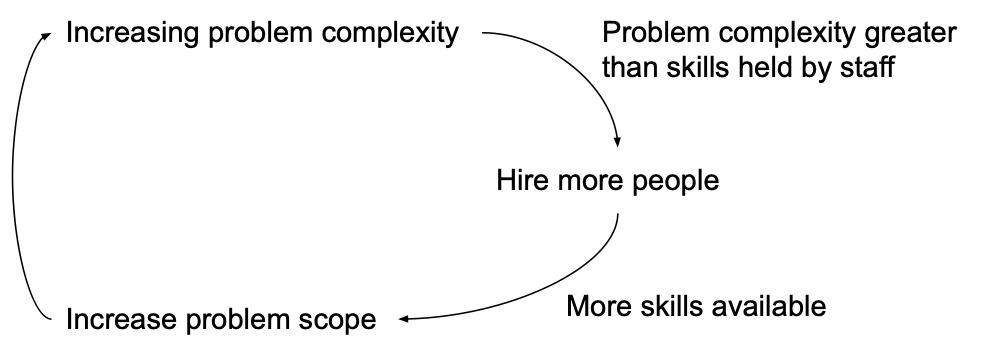
\includegraphics[width=0.8\textwidth]{images/feedback_loop_complexity_and_staffing}
    \caption{Increased complexity requires more staffing to enable specialization. More staff means more skills are available; under-utilized staff skills make room for more scope; more scope adds to complexity.}
    \label{fig:complexity_and_staff_growth}
\end{figure}
\end{center}

% https://graphthinking.blogspot.com/2017/09/a-simple-illustration-of-bureaucracy.html
%\marginpar{[Tag] Story Time}
\index{story time!airport security}
\index{exemplar!Transportation Security Administration@\href{https://en.wikipedia.org/wiki/Transportation_Security_Administration}{Transportation Security Administration (TSA)}}
%\begin{storytime}{Airport Security Line}
\begin{mdframed}[frametitle={Airport Security Line},frametitlerule=true,frametitlealignment=\centering]
A coworker and I were going through passport control at an airport. 
A \href{https://en.wikipedia.org/wiki/Transportation_Security_Administration}{Transportation Security Administration (TSA) officer} 
%\index{exemplar!\href{https://en.wikipedia.org/wiki/Transportation_Security_Administration}{Transportation Security Administration (TSA)}}
\index{Wikipedia!Transportation Security Administration@\href{https://en.wikipedia.org/wiki/Transportation_Security_Administration}{Transportation Security Administration}}
%CANTDOWITHINMDFRAMED\marginpar{$>$Wikipedia: TSA}
was directing passengers into one of two lines. Both lines were long. The length of each line was not equal even though the entrance to the lines was at the same location. Each line terminated at a row of passport-checking agents. Each passport check took a minute. Passport-checking TSA officers operate independently and concurrently.


The TSA officer's perspective is that there are two long lines. Her procedure is to balance the two lines (for fairness). She does this by pointing people into one of the two lines, with her choice driven by which line appears to have room available.

My coworker and I enter the controlled area and are directed into lines by the TSA officer. The officer directs my coworker left and directs me to go right. The TSA officer completed her job.

My coworker in the left line finishes 5 minutes before me. This difference in completion time is frustrating for me.

Because the lines were not of equal length, balancing the start of the line is a suboptimal method. The consequence is that what seems fair to the TSA officer ends up not being fair for people going through the line. The TSA officer had incomplete information -- the lines were not of equal length. Because the TSA officer isn't exposed to the consequence of her approach, she didn't get feedback on whether her decisions are suboptimal or not.
%\end{storytime}
\end{mdframed}

Lesson: if the people making decisions do not experience the consequences of those decisions, then they have no incentive to improve decision-making.

The person in the longer line feels frustrated. The negative feeling is due to a sense of powerlessness, the situation is recurring, and a better solution is available.

The optimal solution in this situation is to have a single line feeding the multiple TSA passport checkers. A single line eliminates the need for the decision-maker but incurs work to change the status quo.


%\subsubsection{Parking garage}
% from
% https://graphthinking.blogspot.com/2019/07/altering-feedback-loops-to-change.html

%\marginpar{[Tag] Story Time}
\index{story time!parking garage}
%\begin{storytime}{Parking Garage}
\begin{mdframed}[frametitle={Parking Garage},frametitlerule=true,frametitlealignment=\centering]
Bob parks his car in a parking garage every day. 
The parking garage owner charges \$20 per day for people to park their car.

Bob recently found that one of the exit gates for the parking garage is broken. If Bob uses that gate to leave the parking garage, the gate does not function and Bob cannot exit. Then Bob has to call the parking gate operator to request an exception (which is granted) and Bob can then exit that gate, avoiding the \$20 per day charge.

This action (go to the broken gate, request an exception, avoid the charge) has been repeated for a long time (months). Bob's motive is to avoid the \$20 parking charge; the cost is a mere phone call and a minor delay. This cheating behavior harms the parking garage owner's income. However, the parking gate operator, serving as intermediary, insulates the parking garage owner from interaction with the cheater. The cheating behavior is small enough that the parking garage owner may not notice.
%\end{storytime}
\end{mdframed}

Having an intermediary policy enforcer alleviates the need for the garage owner to interact with customers. If the incentives of stakeholders are not aligned then inefficiency goes unchecked. If the parking garage operator's profits are a fixed rate rather than tied to parking charges, then the operator lacks the motive to fix problems. 